\Chapter{Understanding Adversarial Influence in Distributed Systems: How can network structure in a distributed system create vulnerabilities to adversarial influence? }\label{ch4}

%\noindent\textbf{\emph{How can network structure in a distributed system create vulnerabilities to adversarial influence?}}

%\section{Introduction}

Engineering and social systems often consist of many agents making decisions based on locally available information. In an engineering system, a distributed decision making strategy can be necessary when communication, computation, or sensing limitations preclude a centralized control strategy. For example, a group of unmanned aircraft performing surveillance in a hostile area may use a distributed control strategy to limit communication and thus remain undetected. Social systems are inherently distributed: individuals typically make decisions based on personal objectives and the behavior of friends and acquaintances. For example, the decision to adopt a recently released technology, such as a new smartphone, may depend both on the quality of the item itself and on friends' choices.

While there are many advantages of distributed decision making, it can create vulnerability to adversarial manipulation.  Adversaries may attempt to influence individual agents by corrupting the information available to them, creating a chain of events which could degrade the system's performance. Work in the area of cyber-physical systems has focused on reducing the potential impact of adversarial interventions through detection mechanisms: detection of attacks in power networks \cite{Hendricks2014}, estimation and control with corrupt sensor data \cite{Fawzi2014, Bai2014}, and monitoring \cite{Pasqualetti2012}. In contrast to this research, our work focuses on characterizing the impact an adversary may have on distributed system dynamics when no mitigation or detection measures are in place.

We use graphical coordination games, introduced in \cite{Cooper1999, Ullmann1977}, to study the impact of adversarial manipulation.  The foundation of a graphical coordination game is a simple two agent coordination game, where each agent must choose between one of two alternatives, $\{x,y\}$, with payoffs depicted by the following payoff matrix which we denote by $u(\cdot)$: 

\begin{center}
\begin{tabular}{r|c|c|}
\multicolumn{1}{r}{}	&\multicolumn{1}{c}{$x$}	&\multicolumn{1}{c}{$y$}\\
\cline{2-3}$x$			&$1+\alpha,\,1+\alpha$	&$0,\,0$\\
\cline{2-3}$y$			&$0,\,0$				&$1,\,1$\\
\cline{2-3}
\end{tabular}\\
\medskip
$2\times 2$ coordination game, $g$, with utilities $u(a_i,a_j),$ $a_i,a_j\in\{x,y\}$, and payoff gain $\alpha>0$
\end{center}
where $\alpha > 0$ defines the relative quality of conventions $(x,x)$ over $(y,y)$.  Both agents prefer to agree on a convention, i.e., $(x,x)$ or $(y,y)$, than disagree, i.e., $(x,y)$ or $(y,x)$, with a preference to agreeing on $(x,x)$.  
The goal of deriving local agent dynamics which lead to the efficient Nash equilibrium $(x,x)$ is challenging because of the existence of the inefficient Nash equilibrium $(y,y)$.  Deviating from $(y,y)$ for an individual agent is accompanied by an immediate payoff loss of $1$ to $0$; hence, myopic agents may be reluctant to deviate, stabilizing the inefficient equilibrium $(y,y)$.

This two player coordination game can be extended to an $n$-player \emph{graphical coordination game}\cite{Kearns2001,Young2011, Montanari2010}, where the interactions between the agents $N=\{1, 2, \dots, n\}$ is described by an underlying graph $\mathcal{G} = (N,E)$ where $E \subseteq N\times N$ denotes the interdependence of agents' objectives.  More formally, an agent's total payoff is the sum of payoffs it receives in the two player games played with its neighbors ${\cal N}_i = \{j \in N : (i,j) \in E\}$, i.e., for a joint decision $a = (a_1, \dots, a_n) \in \{x,y\}^n$, the utility of agent $i$ is
%
\begin{equation}\label{e:original utility}
%
U_i(a_1, \dots, a_n) = \sum_{j \in {\cal N}_i} u(a_i, a_j).
%
\end{equation}
%
Joint actions $\vec{x}:=(x,x,\ldots,x)$ and $\vec{y}:=(y,y,\ldots,y)$, where either all players choose $x$ or all players choose $y$, are Nash equilibria of the game; other equilibria may emerge depending on the structure of graph $\mathcal{G}.$ In any case, $\vec{x}$ is the unique efficient equilibrium, since it maximizes agents' total payoffs.  Graphical coordination games can model both task allocation in engineering systems  as well as the evolution of social convention in marketing scenarios. 
 
The goal in this setting is to prescribe a set of decision-making rules that ensures emergent behavior is aligned with the efficient Nash equilibrium $\vec{x}$ irrespective of the underlying graph ${\cal G}$ and the choice of $\alpha$. Any such rule must be accompanied by a degree of noise (or mistakes) as agents must be enticed to deviate from inefficient Nash equilibrium.  
Log-linear learning \cite{Blume1993, Shah2010} is one distributed decision making rule that selects the efficient equilibrium, $\vec{x}$, in the graphical coordination game described above. Although agents predominantly maximize their utilities under log-linear learning, selection of the efficient equilibrium is achieved by allowing agents to choose suboptimally with some small probability that decreases exponentially with respect to the associated payoff loss. 

The equilibrium selection properties of log-linear learning extend beyond coordination games to the class of potential games \cite{Monderer1996}, which often can be used to model engineering systems where the efficient Nash equilibrium is aligned with the optimal system behavior \cite{Marden2007,Marden2008,Wolpert2001}.  Hence, log-linear learning can be a natural choice for prescribing control laws in many distributed engineering systems \cite{Marden2008,Zhu2009,Goto2010,Staudigl2012,Fox2010}, as well as for analyzing the emergence of conventions in social systems \cite{Young1993,Shah2010}.  This prompts the question: can adversarial manipulation  alter the emergent behavior of log-linear learning in the context of graphical coordination games (or more broadly in distributed engineering systems)?

We study this question in the context of the above graphical coordination games. Here, we model the adversary as additional nodes/edges in our graph, where the action selected by these adversaries (which we fix as the inferior convention $y$) impacts the utility of the neighboring agents and thereby influences the agents' decision-making rule as specified by log-linear learning.  We focus on three different models of adversary behavior, referred to as \emph{fixed, intelligent}; \emph{mobile, random}; and \emph{mobile, intelligent}. 
%
\begin{itemize}
%
\item A fixed intelligent adversary aims to influence a fixed set $S\subseteq N$. To these agents the adversary appears to be a neighbor who always selects alternative  $y$.  We assume that $S$ is selected based on the graph structure ${\cal G}$ and $\alpha$.   
%
\item A mobile, random adversary connects to a random collection of agents $S(t)\subseteq N$ at each time, $t\in \mathbb{N}$ using no information on graph structure, $\mathcal{G},$ or payoff gain, $\alpha.$ 
%
\item A mobile, intelligent agent connects to a collection of agents, $S(t)\subseteq N$, at each time, $t\in \mathbb{N}$ using information on graph structure, $\mathcal{G}$, payoff gain $\alpha$, and the current action profile, $a(t)$.  
%
\end{itemize}
%
We will discuss each type of adversary's influence on an arbitrary graph, and then analyze the worst case influence on a set of agents interacting according to a line. We specify the values of payoff gain $\alpha$ for which an adversary can stabilize joint action $\vec{y}$, showing that a mobile, intelligent agent can typically stabilize joint action $\vec{y}$ for larger values of $\alpha$ than a mobile, random agent, and a mobile, random agent can typically stabilize $\vec{y}$ for larger values of $\alpha$ than a fixed, intelligent agent. 

\section{The model}

Suppose agents in $N$ interact according to the graphical coordination game above, with underlying graph $\mathcal{G} = (N,E)$, alternatives $\{x,y\}$ and payoff gain $\alpha.$ We denote the joint action space by $\mathcal{A} = \{x,y\}^n,$ and we write
$$(a_i,a_{-i}) = (a_1,a_2,\ldots,a_i,\ldots,a_n)\in\mathcal{A}$$
when considering agent $i$'s action separately from other agents' actions.


Now, suppose agents in $N$ update their actions according to the \emph{log-linear learning} algorithm at times $t = 0,1,\ldots,$ producing a sequence of joint actions $a(0),a(1),\ldots$. We assume agents begin with joint action, $a(0)\in\mathcal{A}$, and let $a(t) = (a_i,a_{-i})\in\mathcal{A}.$  At time $t\in\mathbb{N}$, an agent $i\in N$ is selected uniformly at random to update its action for time $t+1$; all other agents' actions will remain fixed. Agent $i$ chooses its next action probabilistically according to:\footnote{Agent $i$'s update probability is also conditioned on the fact that agent $i$ was selected to revise its action, which occurs with probability $1\mathop{/}n$. For notational brevity we omit this throughout, and  $\Pr[a_i(t+1) = A\,|\, a_{-i}(t) = a_{-i}]$, for example, is understood to mean $\Pr[a_i(t+1) = x\,|\, a_{-i}(t) = a_{-i},\, i \text{ selected for update}].$}
%\small
\begin{align}
&\Pr[a_i(t+1) = x\,|\, a_{-i}(t) = a_{-i}]\nonumber \\
&\hspace{.4in}= {\exp \left(\beta \cdot U_i(x,a_{-i})\right)\over \exp \left(\beta \cdot  U_i(x,a_{-i}\right)+\exp \left(\beta \cdot U_i(y,a_{-i})\right)}.\label{e:LLL dynamics}
\end{align} 
Parameter $\beta>0$ dictates an updating agent's degree of rationality. %and is identical for all agents $i\in N$. 
As $\beta\to \infty$, agent $i$ is increasingly likely to select a utility maximizing action, and as $\beta\to 0$, agent $i$ tends to choose its next action uniformly at random.
The joint action at time $t+1$ is
$a(t+1) = (a_i(t+1),a_{-i}(t)).$


Joint action, $a\in\mathcal{A}$ is \emph{strictly stochastically stable} \cite{Foster1990} under log-linear learning dynamics if, for any $\eps >0$, there exist $B<\infty$ and $T<\infty$ such that
\begin{equation}
\Pr[a(t)=a] > 1-\eps,\quad\text{for all } \beta > B, t>T
\end{equation}
where $a(t)$ is the joint action at time $t\in\N$ under log-linear learning dynamics.

Joint action $\vec{x}$ is strictly stochastically stable under log-linear learning dynamics over graphical coordination game $G$ \cite{Blume1993}. We will investigate conditions when an adversary can destabilize $\vec{x}$ and stabilize an alternate equilibrium.



Consider the situation where agents in $N$ interact according to the graphical game $G$, and an adversary seeks to  convert as many agents in $N$ to play action $y$ as possible.\footnote{In this paper we consider a single adversary which may influence multiple agents. Our models can be extended to multiple adversaries whose objectives are either aligned or conflicting.} 
At each time, $t\in \N$ the adversary attempts to influence a set of agents $S(t)\subseteq N$ by posing as a friendly agent who always plays action $y$. Agents' utilities, $\tilde{U}:\mathcal{A}\times 2^N\to\R$, are now a function of adversarial and friendly behavior, defined by:
\begin{equation}\label{e:new utility}
\tilde{U_i}((a_i,a_{-i}),S) = %U_i(a_i,a_{-i}) + \mathds{1}_{i\in S, a_i = y}
\begin{cases}
U_i(a_i,a_{-i})	&\text{if } i\notin S\\
U_i(a_i,a_{-i})	&\text{if } a_i = x\\
U_i(a_i,a_{-i}) + 1 &\text{if } i\in S,  a_i = y 
\end{cases}
\end{equation}
where $(a_i,a_{-i})\in\mathcal{A}$ represents friendly agents' joint action, and $S\subseteq N$ represents the set influenced by the adversary.
If  $i\in S(t)$, agent $i$ receives an additional payoff of 1 for coordinating with the adversary at action $y$ at time $t\in\N$; to agents in $S(t)$ the adversary appears to be a neighbor playing action $y$. By posing as a player in the game, the adversary has manipulated the utilities of agents belonging to $S$, providing an extra incentive to choose the inferior alternative, $y$. 

Suppose agents revise their actions according to log-linear learning as in \eqref{e:LLL dynamics}, where the utility, $U_i$ defined in \eqref{e:original utility} is replaced by $\tilde{U}_i$ in \eqref{e:new utility}. An agent $i\in N$ which revises its action at time $t\in\N$ bases its new action choice on the utility $\tilde{U}_i(a(t),S(t))$ if $i\in S(t)$, increasing the probability that agent $i$ updates its action to $y$. By posing as a player in the coordination game, an adversary manipulates agents' utility functions.thereby modifying their decision making rules.



\section{Summary of results}

In the following sections, we will precisely define three models of adversarial behavior: fixed, intelligent; mobile, random; and mobile, intelligent. Each type of adversary has a fixed capability, $k$, i.e., $|S(t)| = k$ for all $t\in\N.$ 
Our analysis of these models will provide insight into an adversary's influence on a general graph, $\mathcal{G}$, and we derive exact bounds on $\alpha$ for adversarial influence on a line. Values of $\alpha$ for which each type of agent can stabilize $\vec{y}$ in the line are summarized below and in Figure~\ref{f:barGraph}.
\begin{itemize}
\item A fixed, intelligent adversary with capability $k$ can stabilize joint action $\vec{y}$ when $\alpha<k\mathop{/}(n-1)$ (Theorem~\ref{t:fixed line graph}).
\item A mobile, random adversary with capability $k\leq n-1$ can stabilize joint action $\vec{y}$ when $\alpha <1$ (Theorem~\ref{t:mr ss}).
\item A mobile, intelligent adversary with capability $k=1$ can stabilize joint action $\vec{y}$ when $\alpha <1$ (Theorem~\ref{t:intelligent}).
\item A mobile, intelligent adversary with capability $k\geq 2$ can stabilize joint action $\vec{y}$ when $\alpha <n\mathop{/}(n-1)$ (Theorem~\ref{t:intelligent}).
\end{itemize}
Note that a mobile, random adversary's influence is the same for any capability $k$ with $1\leq k\leq n-1.$ Similarly, a mobile, intelligent adversary does not increase its influence on agents in a line by increasing its capability above $k=2.$

\begin{figure}[!]
  \centering
    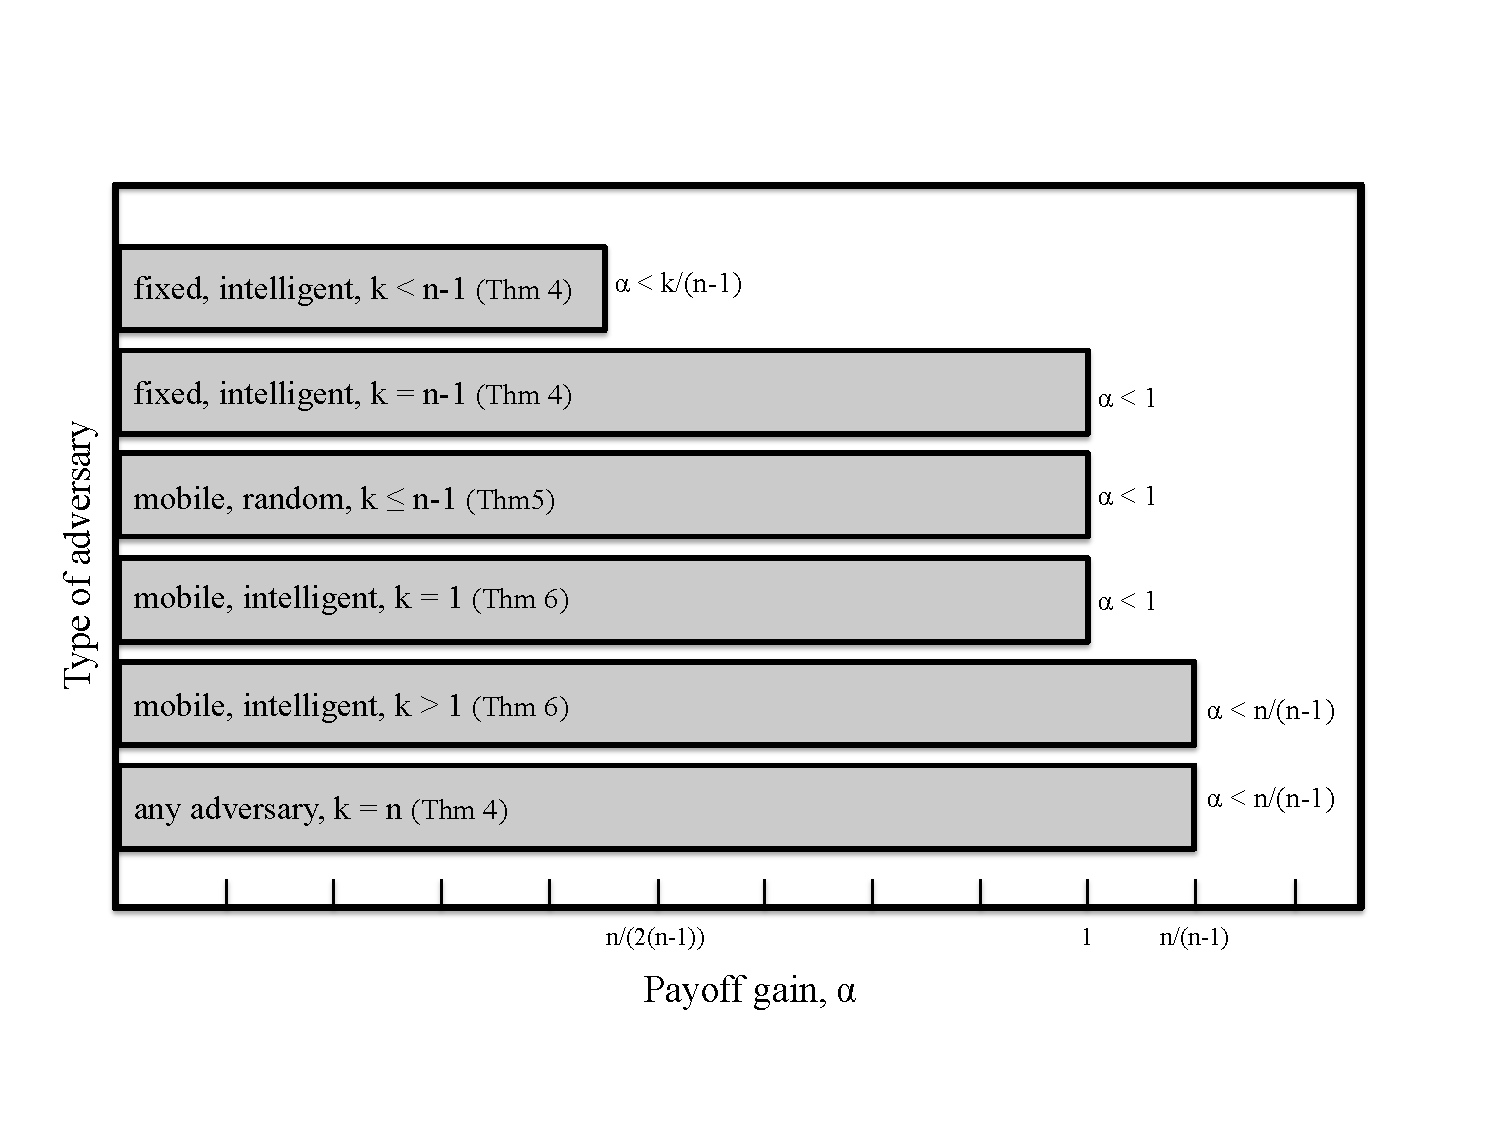
\includegraphics[width=.4\textwidth, clip, trim=10mm 10mm 20mm 30mm]{Presentation2}
  \caption{Values of $\alpha$ for which each type of adversary can stabilize joint action $\vec{y}$ in an $n$-agent line}\label{f:barGraph}
\end{figure}

\section{Main results}
Here, we present a detailed version of the results summarized above. 

\subsection{Universal resilience to an adversary}

A graphical coordination game $G$ is universally resilient to an adversary if $\vec{x}$ is strictly stochastically stable for all possible influenced sets $S(t)$, $t\in N$ and adversarial capability, $k\leq n.$ The following theorem provides sufficient conditions that ensure $G$ is universally resilient. For sets $S,T\subseteq N$, define
$$d(S,T) := |\{\{i,j\}\in E\st i\in S, j\in T\}|.$$

\begin{Theorem}\label{t:A stable all}
Let $\mathcal{G} = (N,E)$, and suppose an adversary influences some set $S(t)$ with $|S(t)| = k$ at each $t\in\N.$ If
\begin{equation}\label{e:YoungBound}
\alpha > {|T| - d(T,N\setminus T)\over d(T,N)},\quad\forall T\subseteq N
\end{equation}
Then $\vec{x}$ is strictly stochastically stable. In particular, if $|S(t)| = N$ for all $t\in \N$, \eqref{e:YoungBound} is also a necessary condition for strict stochastic stability of $\vec{x}$. 
\end{Theorem}

\smallskip

The proof of Theorem~\ref{t:A stable all} follows by using a straightforward adaptation of Proposition 2 in \cite{Young2011} to our adversarial model, included in Appendix~\ref{a:fixed line graph proofs}

When $\alpha$ satisfies \eqref{e:YoungBound}, an adversary cannot influence the game for any $S(t).$ If $\vec{x}$ is strictly stochastically stable when the adversary influences set $S(t)=N$ for all $t\in\N$, then $\vec{x}$ will be strictly stochastically stable for any sequence of influenced sets, $S(t)\subseteq N.$ In this case, game $G$ is resilient in the presence of any adversary with capability $k\leq n$.\footnote{Our results can naturally be extended to a multi-agent scenario. The primary differences occur when multiple adversaries can influence a single friendly agent (or, equivalently, when an adversary's influence is weighted by some factor greater than 1). In this scenario, multiple adversaries can more easily overpower the influence of friendly agents on agent $i$. We will address this in future work.}

When \eqref{e:YoungBound} is satisfied for some $T\subseteq N$, this means that agents in $T$ have a sufficiently large proportion of neighbors in $N$. In this case, $T$ can only be influenced by an adversary when the payoff gain, $\alpha$, is small.

\subsection{Fixed, intelligent adversarial influence}

In the fixed, intelligent model of behavior, the adversary knows graph structure, $\mathcal{G}$, and the value of payoff gain, $\alpha.$ Using this information it influences some fixed subset, 
$$S(t) = S\subseteq N, |S| = k,\quad \forall t\in\N,$$
aiming to maximize the number of agents playing $y$ in a stochastically stable state. Agents in $N$ update their actions according to log-linear learning as in \eqref{e:LLL dynamics} with utilities $$\tilde{U}_i(a(t),S(t)) = \tilde{U}_i(a(t),S),\quad\forall t\in\N.$$ 

We begin with two theorems which provide conditions for stochastic stability in an arbitrary graph $\mathcal{G}$ influenced by an adversary, and then we analyze stability conditions in detail for the line.

\begin{Theorem}\label{t:A stable fixed}
Suppose agents in $N$ are influenced by a fixed, intelligent adversary with capability $k$. Joint action $\vec{x}$ is strictly stochastically stable for any influenced set $S$ with $|S| = k$ if and only if
\begin{equation}
\alpha > {|T\cap S| - d(T,N\setminus T)\over d(T,N)},%,\quad\forall S\subseteq N
%{d(S,N)\over d(S) + |S\cap K|} > {1\over 2+\alpha}
\end{equation}
$\forall T\subseteq N,\,T\neq\emptyset$ and $\forall S\subseteq N$ with $|S| = k$.
\end{Theorem}
%The proof follows similarly to the proof to Theorem~\ref{t:A stable all}.

Theorem~\ref{t:B ss} provides conditions which ensure an adversary can stabilize joint action $\vec{y}$.%for all choices of influenced set, $K$.
\begin{Theorem}\label{t:B ss}
A fixed, intelligent  adversary with capability $k$ can stabilize $\vec{y}$ by influencing set $S\subseteq N$ with $|S|=k$ if and only if
\begin{equation}\label{e:above}
\alpha < {d(T,N\setminus T) + k - |T\cap S|\over d(N\setminus T,N\setminus T)}
%d(N,N) + k > (1+\alpha)d(N\setminus S, N\setminus S) + d(S,S) + |S\cap K|
\end{equation}
for all $T\subseteq N$, $T\neq N$.
\end{Theorem}

The proofs of Theorems~\ref{t:A stable fixed} and \ref{t:B ss} follow similarly to the proof of Theorem~\ref{t:A stable all} and are omitted for brevity.


\noindent\emph{The line:} We now analyze a fixed, intelligent adversary's influence on the line. Let $\mathcal{G} = (N,E)$ with $N = \{1,2,\ldots,n\}$ and $E = \{\{i,j\}:j = i+1\},$ i.e., $\mathcal{G}$ is a line with $n$ nodes. Define 
\begin{align*}
[t] := \{1,2,\ldots,t\}\subseteq N, \text{ and }
[i,j] := \{i,i+1,\ldots,j\}\subseteq N.
\end{align*}


Theorem~\ref{t:fixed line graph} summarizes stability conditions for the line influenced by a fixed, intelligent adversary.

\begin{Theorem}\label{t:fixed line graph}% \blue{still haven't double checked all of these. there may be errors.}
Suppose $\mathcal{G}$ is influenced by a fixed, intelligent adversary with capability $k$. Then:
\begin{enumerate}%[label=(\emph{\alph*})]

\item Joint action $\vec{x}$ is strictly stochastically stable under any influenced set $S\subseteq N$ with $|S| = k$ if and only if
\begin{equation}
\alpha > \max\left\{{k-1\over k},{k\over n-1}\right\}.
\end{equation}


\item If $\alpha <{k\over n-1}$ and the adversary distributes influenced set $S$ as evenly as possible along the line, so that $$\left|S\cap [i,i+t]\right| \leq \left\lceil {kt\over n}\right\rceil$$ for any set of nodes $[i,i+t]\subseteq N$, with $1\leq i \leq n-t,$ $t\leq n$ 
then $\vec{y}$ is strictly stochastically stable.

\item Joint action $\vec{y}$ is strictly stochastically stable for all influenced sets $S$ with $|S| = k$ if and only if
\begin{equation}
\alpha < {1+k-t\over n-t-1},\;\quad\forall t = 1,\ldots,k.
\end{equation}

\item If ${k\over n-1}< \alpha < {k-1\over k},$ the adversary can influence at most
$$t_{\max} = \max\left\{t\st \alpha < {\min\{t,k\}-1\over t}\right\}$$
agents to play $\vec{y}$ in the stochastically stable state by distributing $S$ as evenly as possible along $[t]$, so that
$$|S\cap [i,i+\ell]|\leq \left\lceil {k\ell\over t}\right\rceil \text{ and } S\cap[t+1,n] = \emptyset$$
for any set of nodes $[i,i+\ell]\subset N$ with $1\leq i\leq t-\ell$, and $\ell < t.$

\end{enumerate}

\end{Theorem}

The proof of Theorem~\ref{t:fixed line graph} is in Appendix~\ref{a:fixed line graph proofs}.


\subsection{Mobile, random adversarial influence}

Now, consider an adversary which influences a randomly chosen set $S(t)\subseteq N$ at each $t\in \N.$ The adversary chooses each influenced set, $S(t)$, independently according to a uniform distribution over 
$\mathcal{S}_k:=\{S\in 2^N\st |S| = k\}$
An updating agent $i\in N$ revises according to \eqref{e:LLL dynamics}, where $i\in S(t)$ with probability $k\mathop{/}n$.% and $i\notin S(t)$ with probability $(n-k)\mathop{/}n$. 

\noindent\emph{The line:} 
Suppose a mobile, random adversary attempts to influence a set of agents arranged in a line. Theorem~\ref{t:fixed line graph} addresses the scenario where $k = n,$ since in this case random and fixed agents are equivalent. Hence, Theorem~\ref{t:mr ss} focuses on the case where $1\leq k\leq n-1.$

\begin{Theorem}\label{t:mr ss}
Suppose $\mathcal{G} = (N,E)$ is a line, and agents in $N$ update their actions according to log-linear learning in the presence of a random, mobile adversary with capability $k$, where $1\leq k\leq n-1$. Then joint action $\vec{x}$ is strictly stochastically stable if and only if $\alpha >1,$ and joint action $\vec{y}$ is strictly stochastically stable if and only if $\alpha<1.$ 
\end{Theorem}

Theorem~\ref{t:mr ss} is proved in Appendix~\ref{a:mobile random}.

Note that a mobile, random adversary with capability $k=1$ stabilizes $\vec{y}$ for the same values of $\alpha$ as a mobile, random adversary with any capability $k\leq n-1.$  Recall that a fixed, intelligent adversary with capability $k$ could only stabilize $\vec{y}$ when $\alpha < k\mathop{/} (n-1)$. In this sense, a mobile, random adversary with capability $k=1$ has wider influence than a fixed, intelligent adversary with capability $k\leq n-2.$ 


\subsection{Mobile, intelligent adversarial influence}

Now suppose the adversary chooses $S(t)$ at each $t\in\N$ based on joint action, $a(t)$. We assume a mobile, intelligent adversary with capability $k$ chooses $S(t)$ according to a policy $\mu:\mathcal{A}\to \mathcal{S}_k$ that maximizes the number of agents playing $y$ in a stochastically stable state, given graph structure, $\mathcal{G},$ and payoff gain $\alpha$. 
Again, agents in $N$ update their actions according to log-linear learning as in \eqref{e:LLL dynamics}, with agent $i$'s utility at time $t\in \N$ given by $\tilde{U}_i(a(t),\mu(a(t))$.
We denote the set of optimal adversarial policies for a given capability $k$ by
\begin{equation}
\mathcal{M}_k= \argmax_{\mu\in M_k}\max_{a \text{ stable under }\mu}|\{i\in N\st a_i = y\}|
\end{equation}
where $M_k$ represents the set of all mappings $\mu:\mathcal{A}\to \mathcal{S}_k$, and ``$a$ stable under $\mu$" denotes that joint action $a\in\mathcal{A}$ is strictly stochastically stable under $\mu$. \footnote{Note that the optimal set of policies, $\mathcal{M}_k$, depends highly on the structure of graph $\mathcal{G}$, as does the stationary distribution $\pi^\mu$. In order to maintain notational simplicity, we do not explicitly write this dependence.}



\noindent\emph{The line:} Theorem~\ref{t:intelligent} establishes conditions for strict stochastic stability of joint actions $\vec{x}$ and $ \vec{y}$ in the line influenced by a mobile, intelligent adversary. 


\begin{Theorem}\label{t:intelligent}
Suppose $\mathcal{G} = (N,E)$ is a line, and agents in $N$ update their actions according to log-linear learning. Further suppose a mobile intelligent adversary influences set $S(t)$ at each $t\in \N$ according to an optimal policy for the line, $\mu^\star\in \mathcal{M}_k$. 
\begin{enumerate}%[label=(\emph{\alph*})]
\item If the adversary has capability $k = 1$ then $\vec{x}$ is strictly stochastically stable if and only if $\alpha > 1$, and $\vec{y}$ is strictly stochastically stable if and only if $\alpha <1.$

In particular, when $k=1,$ the policy $\mu^\star:\mathcal{A}\to\mathcal{S}_1$ with:
\begin{equation}\label{e:mustar 1}
\mu^\star(a) = 
\begin{cases}
\{1\} 		&\text{if } a = \vec{x}\\
\{t+1\}		&\text{if } a = (\vec{y}_{[t]},\vec{x}_{[t+1,n]}), \\&\quad\quad t\in \{1,2,\ldots,n-1\}\\
\{1\}			&\text{otherwise}
\end{cases}	
\end{equation}
is optimal, i.e., $\mu^\star\in \mathcal{M}_1$

\item If $2\leq k\leq n$, then $\vec{x}$ is strictly stochastically stable if and only if $\alpha > {n\mathop{/}(n-1)}$, and $\vec{y}$ is strictly stochastically stable if and only if $\alpha < {n\mathop{/} (n-1)}.$


If $2\leq k\leq n-1$, any policy $\mu^\star:\mathcal{A}\to\mathcal{S}_k$ satisfying:
\begin{enumerate}%[label=(\arabic*),leftmargin=1.7em]
\item $1\in\mu^\star(\vec{x})$
\item $1,n\in\mu^\star(\vec{y})$
\item For any $a\in\mathcal{A},\,a\neq \vec{x},\vec{y},$ there exists $i\in \mu^\star(a)$ such that $a_i = x$ and either $a_{i-1} = y$ or $a_{i+1} = y$
\end{enumerate}
is optimal.

\end{enumerate}
\end{Theorem}

The proof of Theorem~\ref{t:intelligent} is included in Appendix~\ref{a:intelligent proof}. Recall that a mobile, random agent with $k\geq 1$ and a fixed, intelligent agent with $k = n-1$ can stabilize $\vec{y}$ any time $\alpha <1;$ an adversary who can intelligently influence a different single agent in $N$ each day can stabilize $\vec{y}$ under these same conditions.  If the intelligent, mobile adversary has capability $k\geq 2$, it can stabilize $ \vec{y}$ when $\alpha < {n\mathop{/} (n-1)}$, i.e., under the same conditions as an adversary with capability $k=n.$

%\section{Summary and future work}

We have shown that a mobile, intelligent adversary with capability $k\geq 2$ can stabilize joint action $\vec{y}$ in a line for any $\alpha < {n\mathop{/}(n-1)}$. Next, an intelligent, mobile adversary with capability $k=1$ and a random, mobile adversary with capability $k\leq n-1$ can stabilize $\vec{y}$ when $\alpha <1$. Finally, a fixed, intelligent adversary with capability $k$ can stabilize $\vec{y}$ when $\alpha < k\mathop{/}(n-1)$. %Figure~\ref{f:barGraph} shows these bounds on $\alpha$ for the 5 agent line graph. 
Recall that a fixed, intelligent adversary can also stabilize a joint action where some subset of agents play action $y$; this only occurs when $\alpha <(\min\{t,k\}-1)\mathop{/} t < 1$ for some $t\leq n$.



In future work, we will address the scenario where multiple adversaries aim to influence agents in $N$.%, or, equivalently, when a single adversary can exert influence on agents with some weight larger than 1. 
By heavily influencing a single agent, adversaries can cause this agent to choose action $y$ with near certainty. Due to cascading effects, this can allow adversaries to stabilize joint action $\vec{y}$ for significantly larger values of payoff gain, $\alpha.$
